% Created by tikzDevice version 0.6.2-92-0ad2792 on 2013-04-07 18:09:46
% !TEX encoding = UTF-8 Unicode
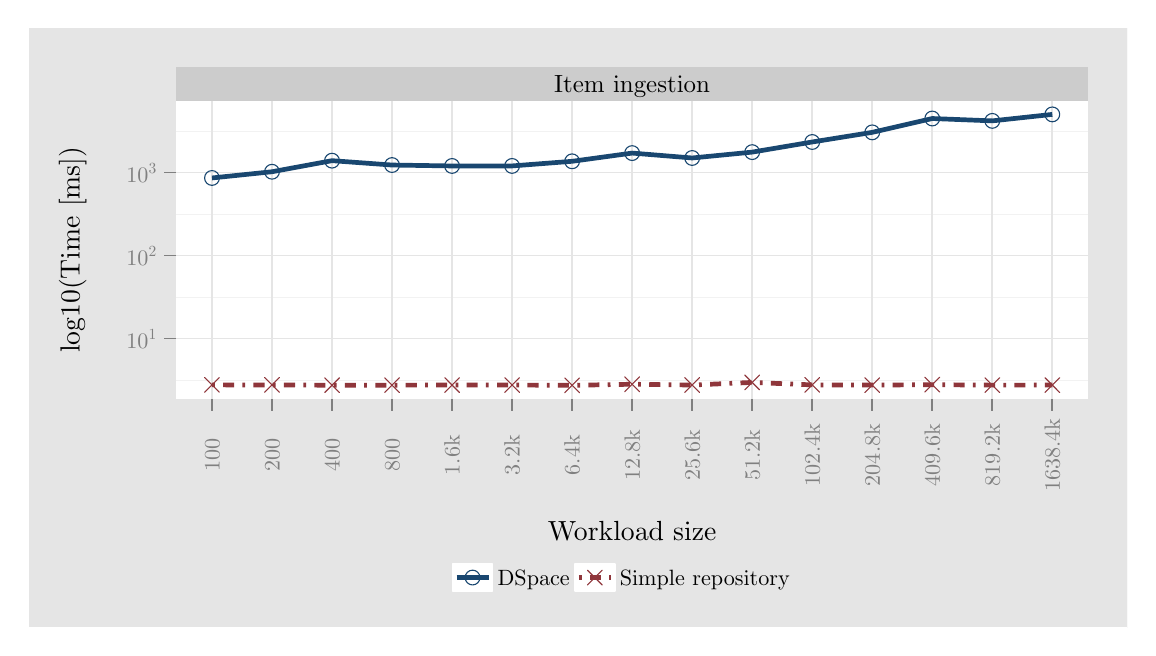
\begin{tikzpicture}[x=1pt,y=1pt]
\definecolor[named]{fillColor}{rgb}{1.00,1.00,1.00}
\path[use as bounding box,fill=fillColor,fill opacity=0.00] (0,0) rectangle (397.48,216.81);
\begin{scope}
\path[clip] (  0.00,  0.00) rectangle (397.48,216.81);
\definecolor[named]{drawColor}{rgb}{1.00,1.00,1.00}
\definecolor[named]{fillColor}{rgb}{0.90,0.90,0.90}

\path[draw=drawColor,line width= 0.6pt,line join=round,line cap=round,fill=fillColor] (  0.00,  0.00) rectangle (397.48,216.81);
\end{scope}
\begin{scope}
\path[clip] ( 53.58, 82.69) rectangle (383.26,190.36);
\definecolor[named]{fillColor}{rgb}{1.00,1.00,1.00}

\path[fill=fillColor] ( 53.58, 82.69) rectangle (383.26,190.36);
\definecolor[named]{drawColor}{rgb}{0.95,0.95,0.95}

\path[draw=drawColor,line width= 0.3pt,line join=round] ( 53.58, 89.48) --
	(383.26, 89.48);

\path[draw=drawColor,line width= 0.3pt,line join=round] ( 53.58,119.46) --
	(383.26,119.46);

\path[draw=drawColor,line width= 0.3pt,line join=round] ( 53.58,149.44) --
	(383.26,149.44);

\path[draw=drawColor,line width= 0.3pt,line join=round] ( 53.58,179.42) --
	(383.26,179.42);
\definecolor[named]{drawColor}{rgb}{0.90,0.90,0.90}

\path[draw=drawColor,line width= 0.6pt,line join=round] ( 53.58,104.47) --
	(383.26,104.47);

\path[draw=drawColor,line width= 0.6pt,line join=round] ( 53.58,134.45) --
	(383.26,134.45);

\path[draw=drawColor,line width= 0.6pt,line join=round] ( 53.58,164.43) --
	(383.26,164.43);

\path[draw=drawColor,line width= 0.6pt,line join=round] ( 66.60, 82.69) --
	( 66.60,190.36);

\path[draw=drawColor,line width= 0.6pt,line join=round] ( 88.29, 82.69) --
	( 88.29,190.36);

\path[draw=drawColor,line width= 0.6pt,line join=round] (109.97, 82.69) --
	(109.97,190.36);

\path[draw=drawColor,line width= 0.6pt,line join=round] (131.66, 82.69) --
	(131.66,190.36);

\path[draw=drawColor,line width= 0.6pt,line join=round] (153.35, 82.69) --
	(153.35,190.36);

\path[draw=drawColor,line width= 0.6pt,line join=round] (175.04, 82.69) --
	(175.04,190.36);

\path[draw=drawColor,line width= 0.6pt,line join=round] (196.73, 82.69) --
	(196.73,190.36);

\path[draw=drawColor,line width= 0.6pt,line join=round] (218.42, 82.69) --
	(218.42,190.36);

\path[draw=drawColor,line width= 0.6pt,line join=round] (240.11, 82.69) --
	(240.11,190.36);

\path[draw=drawColor,line width= 0.6pt,line join=round] (261.80, 82.69) --
	(261.80,190.36);

\path[draw=drawColor,line width= 0.6pt,line join=round] (283.49, 82.69) --
	(283.49,190.36);

\path[draw=drawColor,line width= 0.6pt,line join=round] (305.18, 82.69) --
	(305.18,190.36);

\path[draw=drawColor,line width= 0.6pt,line join=round] (326.87, 82.69) --
	(326.87,190.36);

\path[draw=drawColor,line width= 0.6pt,line join=round] (348.56, 82.69) --
	(348.56,190.36);

\path[draw=drawColor,line width= 0.6pt,line join=round] (370.25, 82.69) --
	(370.25,190.36);
\definecolor[named]{drawColor}{rgb}{0.10,0.28,0.44}

\path[draw=drawColor,line width= 1.7pt,line join=round] ( 66.60,162.50) --
	( 88.29,164.75) --
	(109.97,168.75) --
	(131.66,167.17) --
	(153.35,166.84) --
	(175.04,166.85) --
	(196.73,168.52) --
	(218.42,171.49) --
	(240.11,169.72) --
	(261.80,171.84) --
	(283.49,175.50) --
	(305.18,178.98) --
	(326.87,183.98) --
	(348.56,183.13) --
	(370.25,185.47);
\definecolor[named]{drawColor}{rgb}{0.56,0.21,0.23}

\path[draw=drawColor,line width= 1.7pt,dash pattern=on 1pt off 3pt on 4pt off 3pt ,line join=round] ( 66.60, 87.73) --
	( 88.29, 87.71) --
	(109.97, 87.61) --
	(131.66, 87.63) --
	(153.35, 87.67) --
	(175.04, 87.67) --
	(196.73, 87.58) --
	(218.42, 87.96) --
	(240.11, 87.68) --
	(261.80, 88.62) --
	(283.49, 87.73) --
	(305.18, 87.66) --
	(326.87, 87.80) --
	(348.56, 87.64) --
	(370.25, 87.66);
\definecolor[named]{drawColor}{rgb}{0.10,0.28,0.44}

\path[draw=drawColor,line width= 0.4pt,line join=round,line cap=round] ( 66.60,162.50) circle (  2.67);

\path[draw=drawColor,line width= 0.4pt,line join=round,line cap=round] ( 88.29,164.75) circle (  2.67);

\path[draw=drawColor,line width= 0.4pt,line join=round,line cap=round] (109.97,168.75) circle (  2.67);

\path[draw=drawColor,line width= 0.4pt,line join=round,line cap=round] (131.66,167.17) circle (  2.67);

\path[draw=drawColor,line width= 0.4pt,line join=round,line cap=round] (153.35,166.84) circle (  2.67);

\path[draw=drawColor,line width= 0.4pt,line join=round,line cap=round] (175.04,166.85) circle (  2.67);

\path[draw=drawColor,line width= 0.4pt,line join=round,line cap=round] (196.73,168.52) circle (  2.67);

\path[draw=drawColor,line width= 0.4pt,line join=round,line cap=round] (218.42,171.49) circle (  2.67);

\path[draw=drawColor,line width= 0.4pt,line join=round,line cap=round] (240.11,169.72) circle (  2.67);

\path[draw=drawColor,line width= 0.4pt,line join=round,line cap=round] (261.80,171.84) circle (  2.67);

\path[draw=drawColor,line width= 0.4pt,line join=round,line cap=round] (283.49,175.50) circle (  2.67);

\path[draw=drawColor,line width= 0.4pt,line join=round,line cap=round] (305.18,178.98) circle (  2.67);

\path[draw=drawColor,line width= 0.4pt,line join=round,line cap=round] (326.87,183.98) circle (  2.67);

\path[draw=drawColor,line width= 0.4pt,line join=round,line cap=round] (348.56,183.13) circle (  2.67);

\path[draw=drawColor,line width= 0.4pt,line join=round,line cap=round] (370.25,185.47) circle (  2.67);
\definecolor[named]{drawColor}{rgb}{0.56,0.21,0.23}

\path[draw=drawColor,line width= 0.4pt,line join=round,line cap=round,fill=fillColor] ( 63.93, 85.06) -- ( 69.26, 90.39);

\path[draw=drawColor,line width= 0.4pt,line join=round,line cap=round,fill=fillColor] ( 63.93, 90.39) -- ( 69.26, 85.06);

\path[draw=drawColor,line width= 0.4pt,line join=round,line cap=round,fill=fillColor] ( 85.62, 85.04) -- ( 90.95, 90.38);

\path[draw=drawColor,line width= 0.4pt,line join=round,line cap=round,fill=fillColor] ( 85.62, 90.38) -- ( 90.95, 85.04);

\path[draw=drawColor,line width= 0.4pt,line join=round,line cap=round,fill=fillColor] (107.31, 84.94) -- (112.64, 90.28);

\path[draw=drawColor,line width= 0.4pt,line join=round,line cap=round,fill=fillColor] (107.31, 90.28) -- (112.64, 84.94);

\path[draw=drawColor,line width= 0.4pt,line join=round,line cap=round,fill=fillColor] (129.00, 84.97) -- (134.33, 90.30);

\path[draw=drawColor,line width= 0.4pt,line join=round,line cap=round,fill=fillColor] (129.00, 90.30) -- (134.33, 84.97);

\path[draw=drawColor,line width= 0.4pt,line join=round,line cap=round,fill=fillColor] (150.69, 85.00) -- (156.02, 90.34);

\path[draw=drawColor,line width= 0.4pt,line join=round,line cap=round,fill=fillColor] (150.69, 90.34) -- (156.02, 85.00);

\path[draw=drawColor,line width= 0.4pt,line join=round,line cap=round,fill=fillColor] (172.37, 85.00) -- (177.71, 90.34);

\path[draw=drawColor,line width= 0.4pt,line join=round,line cap=round,fill=fillColor] (172.37, 90.34) -- (177.71, 85.00);

\path[draw=drawColor,line width= 0.4pt,line join=round,line cap=round,fill=fillColor] (194.06, 84.92) -- (199.40, 90.25);

\path[draw=drawColor,line width= 0.4pt,line join=round,line cap=round,fill=fillColor] (194.06, 90.25) -- (199.40, 84.92);

\path[draw=drawColor,line width= 0.4pt,line join=round,line cap=round,fill=fillColor] (215.75, 85.29) -- (221.09, 90.62);

\path[draw=drawColor,line width= 0.4pt,line join=round,line cap=round,fill=fillColor] (215.75, 90.62) -- (221.09, 85.29);

\path[draw=drawColor,line width= 0.4pt,line join=round,line cap=round,fill=fillColor] (237.44, 85.02) -- (242.78, 90.35);

\path[draw=drawColor,line width= 0.4pt,line join=round,line cap=round,fill=fillColor] (237.44, 90.35) -- (242.78, 85.02);

\path[draw=drawColor,line width= 0.4pt,line join=round,line cap=round,fill=fillColor] (259.13, 85.95) -- (264.47, 91.29);

\path[draw=drawColor,line width= 0.4pt,line join=round,line cap=round,fill=fillColor] (259.13, 91.29) -- (264.47, 85.95);

\path[draw=drawColor,line width= 0.4pt,line join=round,line cap=round,fill=fillColor] (280.82, 85.06) -- (286.16, 90.40);

\path[draw=drawColor,line width= 0.4pt,line join=round,line cap=round,fill=fillColor] (280.82, 90.40) -- (286.16, 85.06);

\path[draw=drawColor,line width= 0.4pt,line join=round,line cap=round,fill=fillColor] (302.51, 84.99) -- (307.84, 90.33);

\path[draw=drawColor,line width= 0.4pt,line join=round,line cap=round,fill=fillColor] (302.51, 90.33) -- (307.84, 84.99);

\path[draw=drawColor,line width= 0.4pt,line join=round,line cap=round,fill=fillColor] (324.20, 85.13) -- (329.53, 90.47);

\path[draw=drawColor,line width= 0.4pt,line join=round,line cap=round,fill=fillColor] (324.20, 90.47) -- (329.53, 85.13);

\path[draw=drawColor,line width= 0.4pt,line join=round,line cap=round,fill=fillColor] (345.89, 84.97) -- (351.22, 90.31);

\path[draw=drawColor,line width= 0.4pt,line join=round,line cap=round,fill=fillColor] (345.89, 90.31) -- (351.22, 84.97);

\path[draw=drawColor,line width= 0.4pt,line join=round,line cap=round,fill=fillColor] (367.58, 84.99) -- (372.91, 90.33);

\path[draw=drawColor,line width= 0.4pt,line join=round,line cap=round,fill=fillColor] (367.58, 90.33) -- (372.91, 84.99);
\end{scope}
\begin{scope}
\path[clip] (  0.00,  0.00) rectangle (397.48,216.81);
\definecolor[named]{fillColor}{rgb}{0.80,0.80,0.80}

\path[fill=fillColor] ( 53.58,190.36) rectangle (383.26,202.58);
\definecolor[named]{drawColor}{rgb}{0.00,0.00,0.00}

\node[text=drawColor,anchor=base,inner sep=0pt, outer sep=0pt, scale=  0.90] at (218.42,193.37) {Item ingestion};
\end{scope}
\begin{scope}
\path[clip] (  0.00,  0.00) rectangle (397.48,216.81);
\definecolor[named]{drawColor}{rgb}{0.50,0.50,0.50}

\node[text=drawColor,anchor=base west,inner sep=0pt, outer sep=0pt, scale=  0.80] at ( 35.67,101.04) {10};

\node[text=drawColor,anchor=base west,inner sep=0pt, outer sep=0pt, scale=  0.56] at ( 43.67,104.31) {1};

\node[text=drawColor,anchor=base west,inner sep=0pt, outer sep=0pt, scale=  0.80] at ( 35.67,131.02) {10};

\node[text=drawColor,anchor=base west,inner sep=0pt, outer sep=0pt, scale=  0.56] at ( 43.67,134.29) {2};

\node[text=drawColor,anchor=base west,inner sep=0pt, outer sep=0pt, scale=  0.80] at ( 35.67,161.00) {10};

\node[text=drawColor,anchor=base west,inner sep=0pt, outer sep=0pt, scale=  0.56] at ( 43.67,164.27) {3};
\end{scope}
\begin{scope}
\path[clip] (  0.00,  0.00) rectangle (397.48,216.81);
\definecolor[named]{drawColor}{rgb}{0.50,0.50,0.50}

\path[draw=drawColor,line width= 0.6pt,line join=round] ( 49.31,104.47) --
	( 53.58,104.47);

\path[draw=drawColor,line width= 0.6pt,line join=round] ( 49.31,134.45) --
	( 53.58,134.45);

\path[draw=drawColor,line width= 0.6pt,line join=round] ( 49.31,164.43) --
	( 53.58,164.43);
\end{scope}
\begin{scope}
\path[clip] (  0.00,  0.00) rectangle (397.48,216.81);
\definecolor[named]{drawColor}{rgb}{0.50,0.50,0.50}

\path[draw=drawColor,line width= 0.6pt,line join=round] ( 66.60, 78.42) --
	( 66.60, 82.69);

\path[draw=drawColor,line width= 0.6pt,line join=round] ( 88.29, 78.42) --
	( 88.29, 82.69);

\path[draw=drawColor,line width= 0.6pt,line join=round] (109.97, 78.42) --
	(109.97, 82.69);

\path[draw=drawColor,line width= 0.6pt,line join=round] (131.66, 78.42) --
	(131.66, 82.69);

\path[draw=drawColor,line width= 0.6pt,line join=round] (153.35, 78.42) --
	(153.35, 82.69);

\path[draw=drawColor,line width= 0.6pt,line join=round] (175.04, 78.42) --
	(175.04, 82.69);

\path[draw=drawColor,line width= 0.6pt,line join=round] (196.73, 78.42) --
	(196.73, 82.69);

\path[draw=drawColor,line width= 0.6pt,line join=round] (218.42, 78.42) --
	(218.42, 82.69);

\path[draw=drawColor,line width= 0.6pt,line join=round] (240.11, 78.42) --
	(240.11, 82.69);

\path[draw=drawColor,line width= 0.6pt,line join=round] (261.80, 78.42) --
	(261.80, 82.69);

\path[draw=drawColor,line width= 0.6pt,line join=round] (283.49, 78.42) --
	(283.49, 82.69);

\path[draw=drawColor,line width= 0.6pt,line join=round] (305.18, 78.42) --
	(305.18, 82.69);

\path[draw=drawColor,line width= 0.6pt,line join=round] (326.87, 78.42) --
	(326.87, 82.69);

\path[draw=drawColor,line width= 0.6pt,line join=round] (348.56, 78.42) --
	(348.56, 82.69);

\path[draw=drawColor,line width= 0.6pt,line join=round] (370.25, 78.42) --
	(370.25, 82.69);
\end{scope}
\begin{scope}
\path[clip] (  0.00,  0.00) rectangle (397.48,216.81);
\definecolor[named]{drawColor}{rgb}{0.50,0.50,0.50}

\node[text=drawColor,rotate= 90.00,anchor=base,inner sep=0pt, outer sep=0pt, scale=  0.80] at ( 69.35, 62.36) {100};

\node[text=drawColor,rotate= 90.00,anchor=base,inner sep=0pt, outer sep=0pt, scale=  0.80] at ( 91.04, 62.36) {200};

\node[text=drawColor,rotate= 90.00,anchor=base,inner sep=0pt, outer sep=0pt, scale=  0.80] at (112.73, 62.36) {400};

\node[text=drawColor,rotate= 90.00,anchor=base,inner sep=0pt, outer sep=0pt, scale=  0.80] at (134.42, 62.36) {800};

\node[text=drawColor,rotate= 90.00,anchor=base,inner sep=0pt, outer sep=0pt, scale=  0.80] at (156.11, 62.36) {1.6k};

\node[text=drawColor,rotate= 90.00,anchor=base,inner sep=0pt, outer sep=0pt, scale=  0.80] at (177.80, 62.36) {3.2k};

\node[text=drawColor,rotate= 90.00,anchor=base,inner sep=0pt, outer sep=0pt, scale=  0.80] at (199.49, 62.36) {6.4k};

\node[text=drawColor,rotate= 90.00,anchor=base,inner sep=0pt, outer sep=0pt, scale=  0.80] at (221.18, 62.36) {12.8k};

\node[text=drawColor,rotate= 90.00,anchor=base,inner sep=0pt, outer sep=0pt, scale=  0.80] at (242.86, 62.36) {25.6k};

\node[text=drawColor,rotate= 90.00,anchor=base,inner sep=0pt, outer sep=0pt, scale=  0.80] at (264.55, 62.36) {51.2k};

\node[text=drawColor,rotate= 90.00,anchor=base,inner sep=0pt, outer sep=0pt, scale=  0.80] at (286.24, 62.36) {102.4k};

\node[text=drawColor,rotate= 90.00,anchor=base,inner sep=0pt, outer sep=0pt, scale=  0.80] at (307.93, 62.36) {204.8k};

\node[text=drawColor,rotate= 90.00,anchor=base,inner sep=0pt, outer sep=0pt, scale=  0.80] at (329.62, 62.36) {409.6k};

\node[text=drawColor,rotate= 90.00,anchor=base,inner sep=0pt, outer sep=0pt, scale=  0.80] at (351.31, 62.36) {819.2k};

\node[text=drawColor,rotate= 90.00,anchor=base,inner sep=0pt, outer sep=0pt, scale=  0.80] at (373.00, 62.36) {1638.4k};
\end{scope}
\begin{scope}
\path[clip] (  0.00,  0.00) rectangle (397.48,216.81);
\definecolor[named]{drawColor}{rgb}{0.00,0.00,0.00}

\node[text=drawColor,anchor=base,inner sep=0pt, outer sep=0pt, scale=  1.00] at (218.42, 31.41) {Workload size};
\end{scope}
\begin{scope}
\path[clip] (  0.00,  0.00) rectangle (397.48,216.81);
\definecolor[named]{drawColor}{rgb}{0.00,0.00,0.00}

\node[text=drawColor,rotate= 90.00,anchor=base,inner sep=0pt, outer sep=0pt, scale=  1.00] at ( 18.80,136.53) {log10(Time [ms])};
\end{scope}
\begin{scope}
\path[clip] (  0.00,  0.00) rectangle (397.48,216.81);
\definecolor[named]{fillColor}{rgb}{0.90,0.90,0.90}

\path[fill=fillColor] (145.65,  8.87) rectangle (291.19, 27.36);
\end{scope}
\begin{scope}
\path[clip] (  0.00,  0.00) rectangle (397.48,216.81);
\definecolor[named]{drawColor}{rgb}{1.00,1.00,1.00}
\definecolor[named]{fillColor}{rgb}{1.00,1.00,1.00}

\path[draw=drawColor,line width= 0.6pt,line join=round,line cap=round,fill=fillColor] (153.53, 13.14) rectangle (167.98, 23.09);
\end{scope}
\begin{scope}
\path[clip] (  0.00,  0.00) rectangle (397.48,216.81);
\definecolor[named]{drawColor}{rgb}{0.10,0.28,0.44}

\path[draw=drawColor,line width= 1.7pt,line join=round] (154.98, 18.11) -- (166.54, 18.11);
\end{scope}
\begin{scope}
\path[clip] (  0.00,  0.00) rectangle (397.48,216.81);
\definecolor[named]{drawColor}{rgb}{0.10,0.28,0.44}

\path[draw=drawColor,line width= 0.4pt,line join=round,line cap=round] (160.76, 18.11) circle (  2.67);
\end{scope}
\begin{scope}
\path[clip] (  0.00,  0.00) rectangle (397.48,216.81);
\definecolor[named]{drawColor}{rgb}{1.00,1.00,1.00}
\definecolor[named]{fillColor}{rgb}{1.00,1.00,1.00}

\path[draw=drawColor,line width= 0.6pt,line join=round,line cap=round,fill=fillColor] (197.70, 13.14) rectangle (212.16, 23.09);
\end{scope}
\begin{scope}
\path[clip] (  0.00,  0.00) rectangle (397.48,216.81);
\definecolor[named]{drawColor}{rgb}{0.56,0.21,0.23}

\path[draw=drawColor,line width= 1.7pt,dash pattern=on 1pt off 3pt on 4pt off 3pt ,line join=round] (199.15, 18.11) -- (210.71, 18.11);
\end{scope}
\begin{scope}
\path[clip] (  0.00,  0.00) rectangle (397.48,216.81);
\definecolor[named]{drawColor}{rgb}{0.56,0.21,0.23}
\definecolor[named]{fillColor}{rgb}{1.00,1.00,1.00}

\path[draw=drawColor,line width= 0.4pt,line join=round,line cap=round,fill=fillColor] (202.26, 15.45) -- (207.60, 20.78);

\path[draw=drawColor,line width= 0.4pt,line join=round,line cap=round,fill=fillColor] (202.26, 20.78) -- (207.60, 15.45);
\end{scope}
\begin{scope}
\path[clip] (  0.00,  0.00) rectangle (397.48,216.81);
\definecolor[named]{drawColor}{rgb}{0.00,0.00,0.00}

\node[text=drawColor,anchor=base west,inner sep=0pt, outer sep=0pt, scale=  0.80] at (169.79, 15.36) {DSpace};
\end{scope}
\begin{scope}
\path[clip] (  0.00,  0.00) rectangle (397.48,216.81);
\definecolor[named]{drawColor}{rgb}{0.00,0.00,0.00}

\node[text=drawColor,anchor=base west,inner sep=0pt, outer sep=0pt, scale=  0.80] at (213.96, 15.36) {Simple repository $\;\;\;\;$};
\end{scope}
\end{tikzpicture}
